\chapter{Total above-ground volume\label{chap::total_v}}

In this section, I explore two possible paths to estimate the total above-ground volume, \( \Vtot \). The first option, based on \cite{Longuetaud2013}, uses the ratio:
\begin{equation}
	r = \frac{\Vbole}{\Vtot} \label{eq::r_boletot}
\end{equation}
and is comprised between 0 and 1 by construction. The second option is to fit a multivariate normal distribution, \( \MVN \), to the \textit{transformed} ratio, \( \logit(r) \), jointly with the log-transformed total volume, \( \log(\Vtot) \):
\begin{equation}
	\begin{pmatrix}
		\logit(r) \\
		\log(\Vtot)
	\end{pmatrix}
	\sim
	\MVN\left\{ \begin{pmatrix}
		f(c, \, h; \symbfup{\theta}) \\
		g(c, \, h; \symbfup{\theta}) \\
	\end{pmatrix}, \Sigmabf \right\},
	\label{eq::mvn}
\end{equation}
where \( f \) and \( g \) are functions tailored to our specific needs, \( c \) is circumference at breast height, \( h \), is tree height, and \( \theta \) is a vector of parameters to estimate.

\section{Ratio approach}

I modelled the ratio \( r \) (see equation \eqref{eq::r_boletot}), which quantifies the percentage of volume represented by the bole, by a Beta-distribution. This distribution respects the bounds and accounts for heteroskedasticity, but its parameters \( \text{shape}_1 \) and \( \text{shape}_2 \) are not intuitive. Hence, I reparametrised the Beta-distribution in function of its mean, \( \mu \) and precision, \( \phi \):
\begin{align*}
	\text{shape}_1 &= \phi \mu \\
	\text{shape}_2 &= \phi (1 - \mu)
\end{align*}

Employing the mean and variance is not advisable, since it introduces the interacting constraint \( \sigma^2 < \mu (1 - \mu) \), while the precision lies between 0 and \( + \infty \). The ratio approach has been tested on the 17\textup{th} most common species in the Emerge dataset. The mean \( \mu \) is a function of three parameters to estimate (see equation \eqref{eq::mu-ratio}) and \( \Vbole \), the \textit{predictive variable}:
\begin{equation}
	\mu(\Vbole; \alpha, \beta, \gamma) = \exp[-\beta \Vbole] (\Vbole - \alpha) + \gamma \Vbole + \alpha,
	\label{eq::mu-ratio}
\end{equation}
where \( \alpha, \, \beta\) and \( \gamma \) are parameters to estimate. The results are displayed for \textit{Abies alba} and \textit{Fagus sylvatica}, to represent both conifers and broadleaves (see Fig. \ref{fig::res-mu-ratio}).

\begin{figure}[htb]
	\centering
	\setkeys{Gin}{width=\linewidth}
	\begin{subfigure}{0.4\textwidth}
		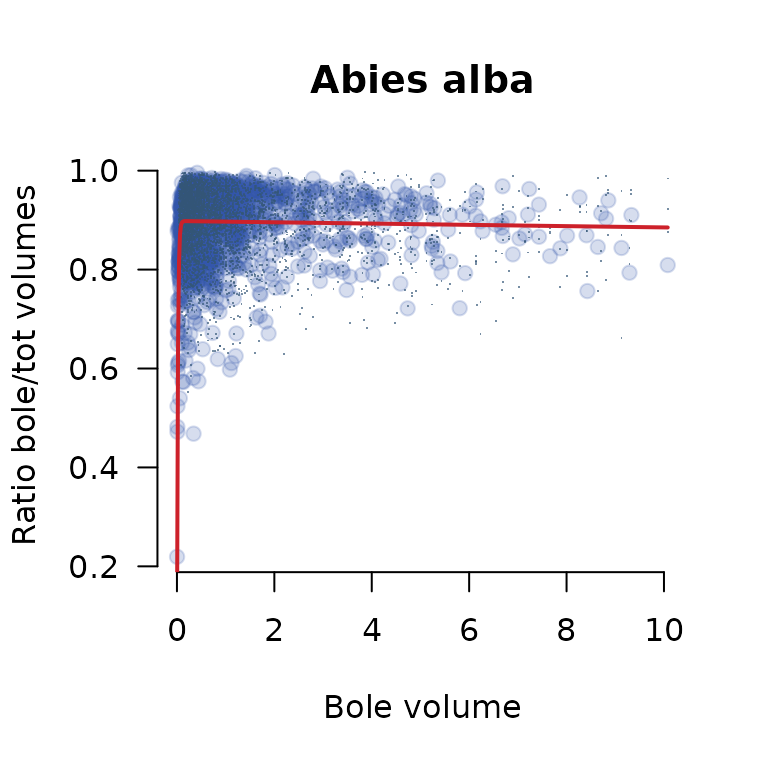
\includegraphics{./Figures/abiesAlba.png}
		\caption{\textit{Abies alba}}
	\end{subfigure}
	\hfil
	\begin{subfigure}{0.4\textwidth}
		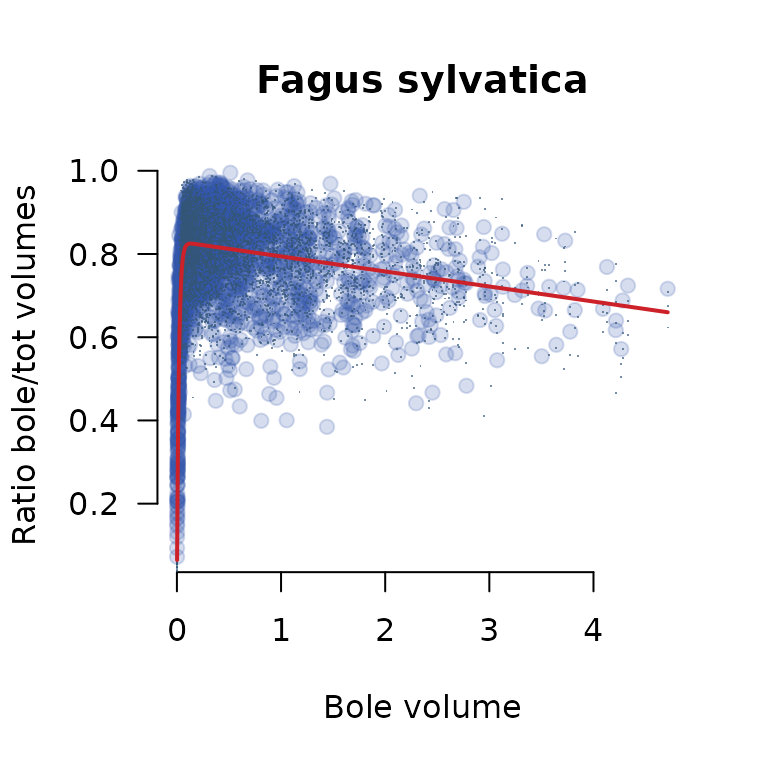
\includegraphics{./Figures/fagSyl.png}
		\caption{\textit{Fagus sylvatica}}
	\end{subfigure}
	\caption{Fit of the ratio data from Emerge only (circles). The dots are posterior predictions, which are in the range of the observations, although residuals show under-dispersion for small values of \( \Vbole \) (see appendix \ref{app::residuals}). The red curve is the fitted equation \eqref{eq::mu-ratio}}
	\label{fig::res-mu-ratio}
\end{figure}

The equation \eqref{eq::mu-ratio} gives similar predictions (see \ref{fig::pred-ratio}) to \cite{Vallet2006} (currently in use at the \NFI) or Emerge\sidenote{In addition to digitising the dataset related to the `Protocole Oudin', the Emerge project aimed to develop a unified allometry for all tree species in French forests. They arrived at the allometry \[ \Vtot = \frac{c^2 h}{4 \pi (1 - \sfrac{1.3}{h})} \left( \alpha + \beta \frac{\sqrt{c}}{h} + \gamma \frac{h}{c} \right).\]This allometry is not used officially by the French \NFI} \parencite{Deleuze2014}. Responses for the non-displayed species are similar to \textit{Abies alba} and \textit{Fagus sylvatica} results.
\begin{figure}[h]
	\centering
	\setkeys{Gin}{width=\linewidth}
	\begin{subfigure}{0.4\textwidth}
		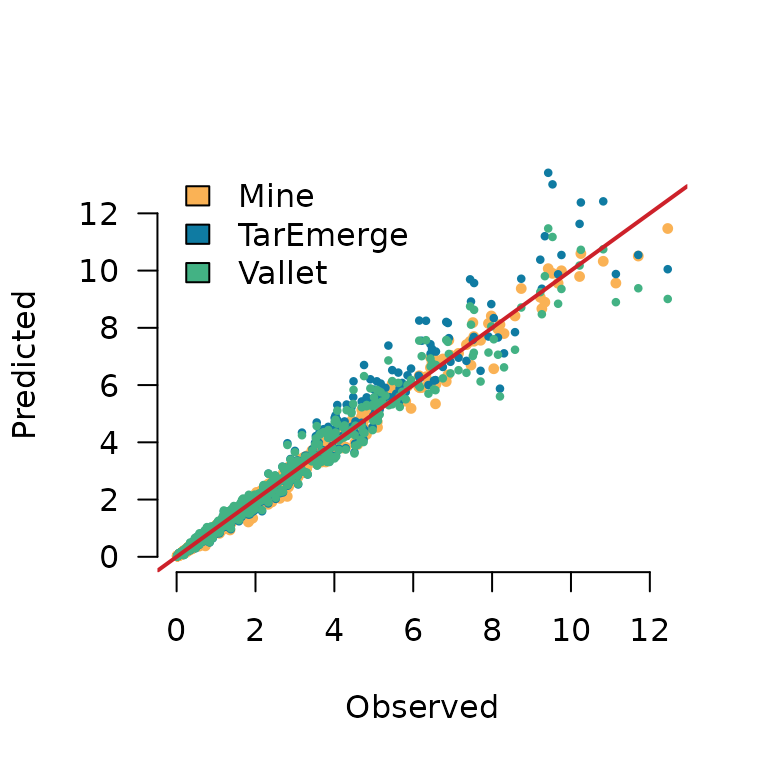
\includegraphics{./Figures/abiesAlba-pred.png}
		\caption{\textit{Abies alba}}
	\end{subfigure}
	\hfil
	\begin{subfigure}{0.4\textwidth}
		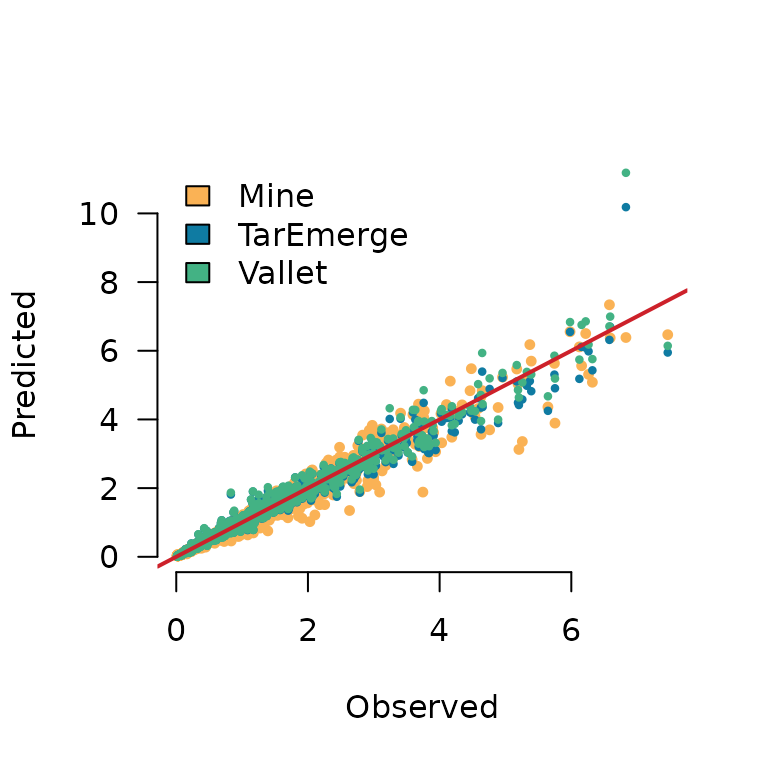
\includegraphics{./Figures/fagSyl-pred.png}
		\caption{\textit{Fagus sylvatica}}
	\end{subfigure}
	\caption{Predictions of total aerial volume in function of bole volume (the explanatory variable) with my model (equation \eqref{eq::mu-ratio}), the current model used at the French \NFI \parencite{Vallet2006}, and the allometry developed during the project Emerge.}
	\label{fig::pred-ratio}
\end{figure}

\section{Multivariate approach}

Multivariate models allow pulling information across components, \ie they describe the variation within and covariation among tree components. I chose to model jointly \( r \) and \( \Vtot \) but the alternative modelling bole and crown could also be considered.

\begin{tcolorbox}[breakable, title = Intractability]
Note that whatever I try to model, there will always be intractability somewhere. If I model both components -- trunk and crown -- with a multivariate lognormal, the distribution of the total volume becomes intractable (sum of two lognormals has no closed form distribution). Alternatively, if I model the total volume and the ratio \( r \) with transformations, then \( \Vbole \) has no closed-form expression. Indeed, to know the product \( \Vbole = r\Vtot \) requires to know the joined distribution of \( r \) and \( \Vtot \).
\end{tcolorbox}

\subsection{Simulated data}
In order to demonstrate the relevance of multivariate methods, I simulate two correlated random variables and then recover the generating parameters. Let \( X \) be an explanatory variable, and \( \mathbf{Y} = (Y_1, \, Y_2) \) be the dependant variable, such that:
\[
	\begin{pmatrix}
		Y_1 \\
		Y_2
	\end{pmatrix} \sim
	\MVN\left\{ \begin{pmatrix}
		\alpha_1 + \beta_1 X \\
		\alpha_2 + \beta_2 X \\
	\end{pmatrix}, \Sigmabf \right\},
\]
where \( \alpha \) and \( \beta \) are regression parameters to estimate, and \( \Sigmabf \) is the variance-covariance matrix defined by:
\[
	\Sigmabf = \begin{bmatrix}
		\sigma_1^2 & \rho \sigma_1 \sigma_2 \\
		\rho \sigma_1 \sigma_2 & \sigma_2^2
	\end{bmatrix}. \\
\]

I am able to recover the parameters \( \alpha \), \( \beta \) and the variance-covariance matrix \( \Sigmabf \) with both a multivariate normal or two separated linear regression as shown in Fig \ref{fig::res-params}. However, when multiplying both variables \( Y_1 \) and \( Y_2 \), as we would do to compute the bole volume from the total volume and the ratio \( r \), we see that the two separated linear models give a biased result with a smaller credibility interval (see Figs. \ref{fig::res-15} -- \ref{fig::res-85}). This is because the real expected value for the product is \( \E[Y_1 Y_2] = \E[Y_1] \E[Y_2] + \Cov[Y_1, Y_2] \) in the correlated case, while for the uncorrelated case it assumes \( \E[Y_1 Y_2] = \E[Y_1] \E[Y_2] \) (since the covariance is \num{0} in this case). The R code is available on \href{https://github.com/amael-ls/emerge/tree/main/communications/cst/2025-10-30/code}{\faIcon{github} Github}. \\

In this simulated case, the principal drawback of employing a \textit{classical} rather than a \textit{multivariate} model is that it produces narrower credibility intervals and apparently consistent parameter estimates, yet leads to a biased output product \( Y_1 Y_2\).

\begin{figure}[htb]
	\centering
	\setkeys{Gin}{width=\linewidth}
	\begin{subfigure}{0.4\textwidth}
		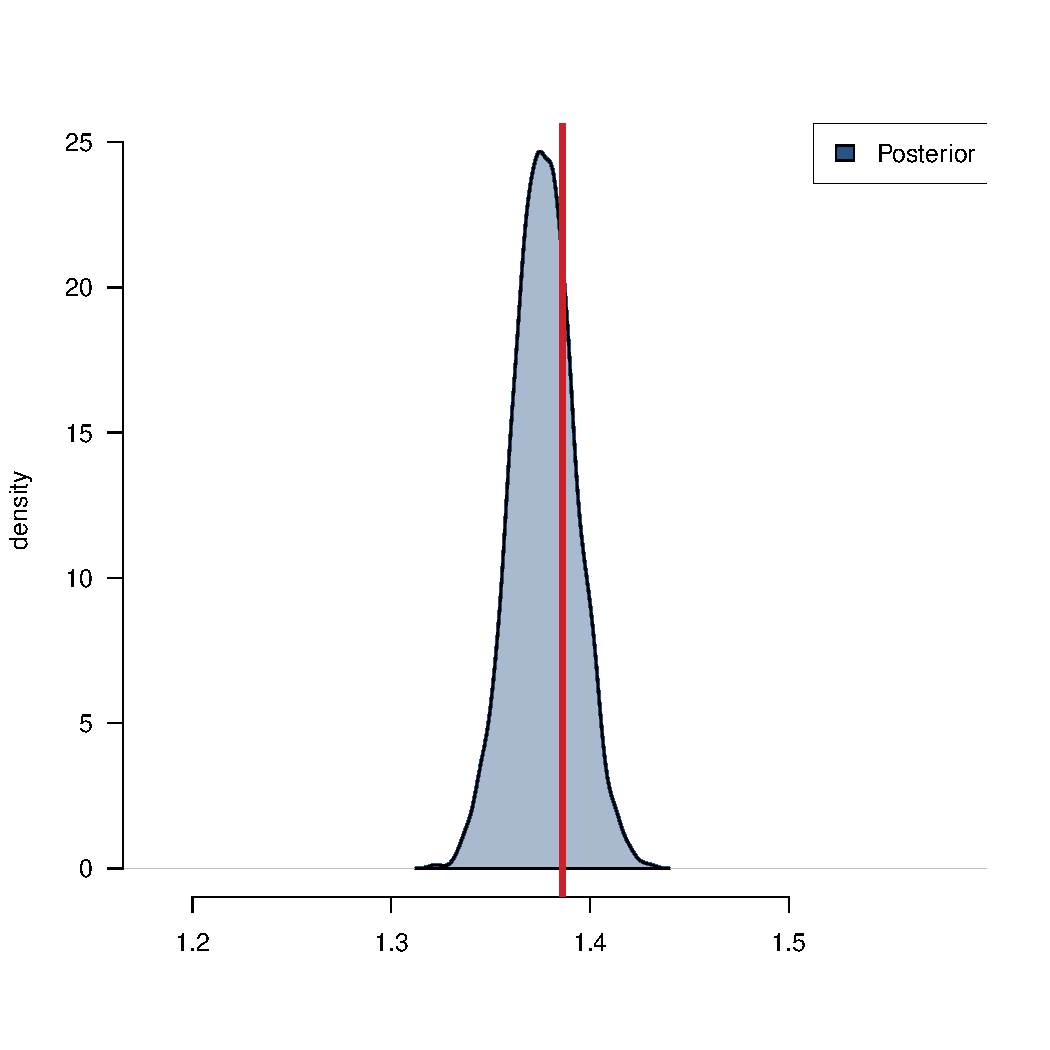
\includegraphics{./Figures/alpha_corr.pdf}
		\caption{Multivariate model}
	\end{subfigure}
	\hfil
	\begin{subfigure}{0.4\textwidth}
		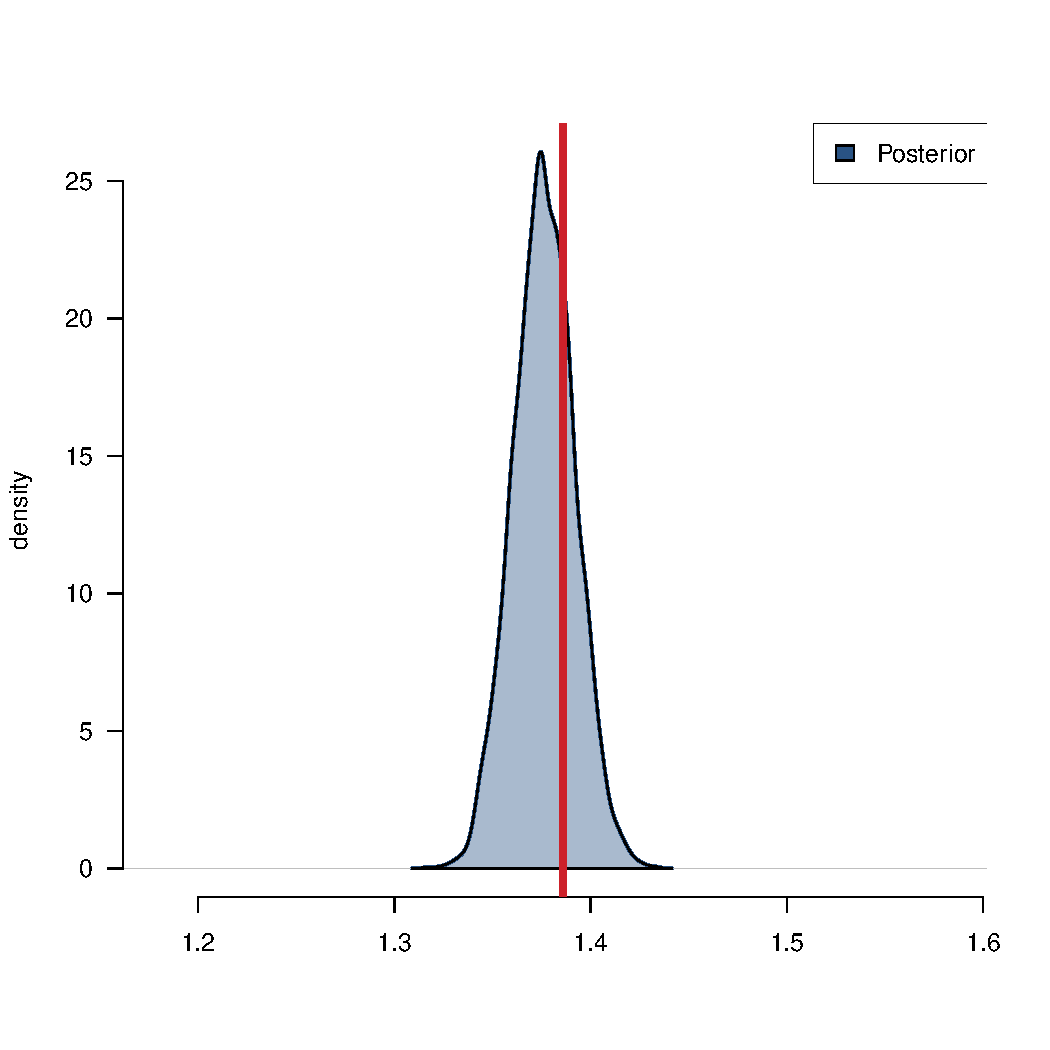
\includegraphics{./Figures/alpha_uncorr.pdf}
		\caption{Uncorrelated model}
	\end{subfigure}
	\caption{Posterior of the intercept parameter \( \alpha \), with the real value displayed in red. As can be seen, both model can recover the intercept (and same for the other parameters)}
	\label{fig::res-params}
\end{figure}


\begin{figure}[htb]
	\centering
	\setkeys{Gin}{width=\linewidth}
	\begin{subfigure}{0.4\textwidth}
		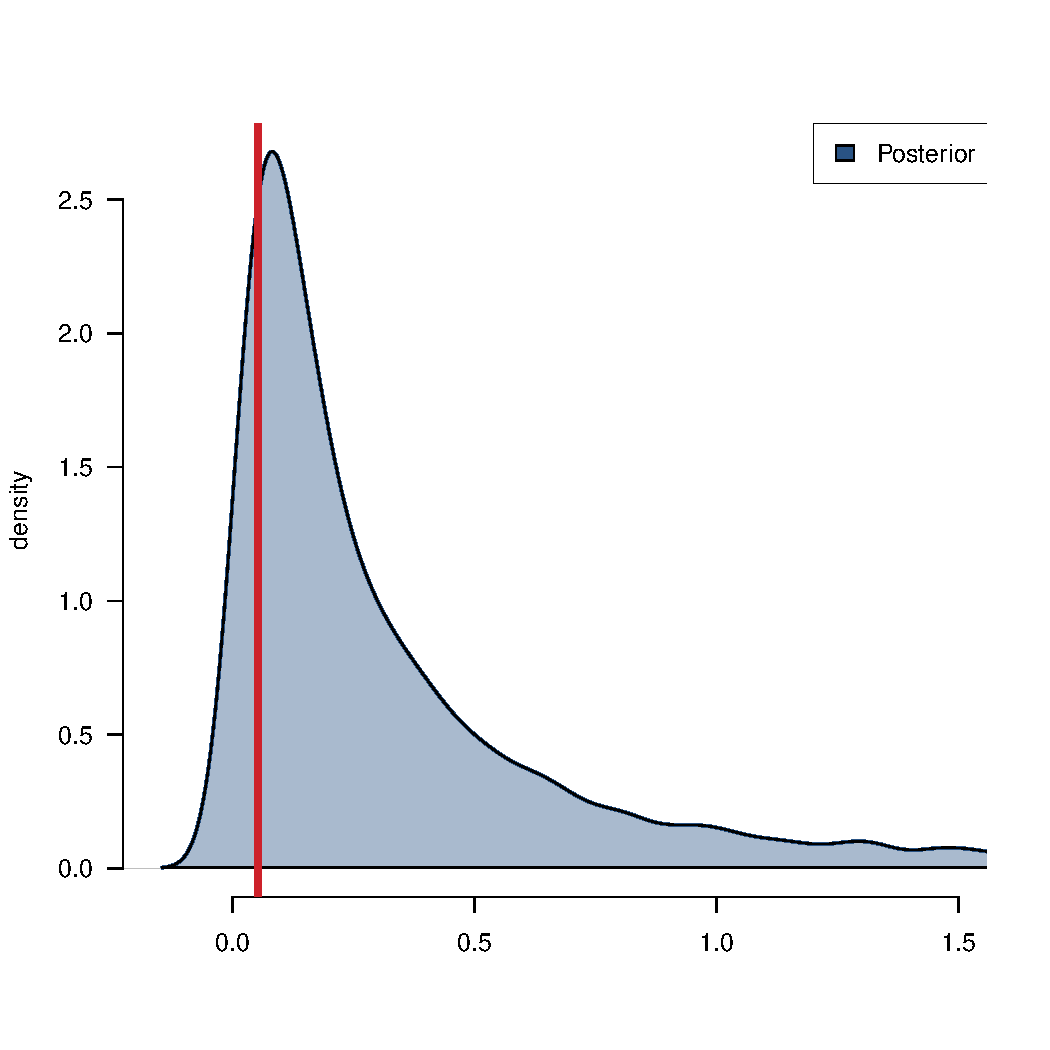
\includegraphics{./Figures/15th-percentile_corr.pdf}
		\caption{Multivariate model}
	\end{subfigure}
	\hfil
	\begin{subfigure}{0.4\textwidth}
		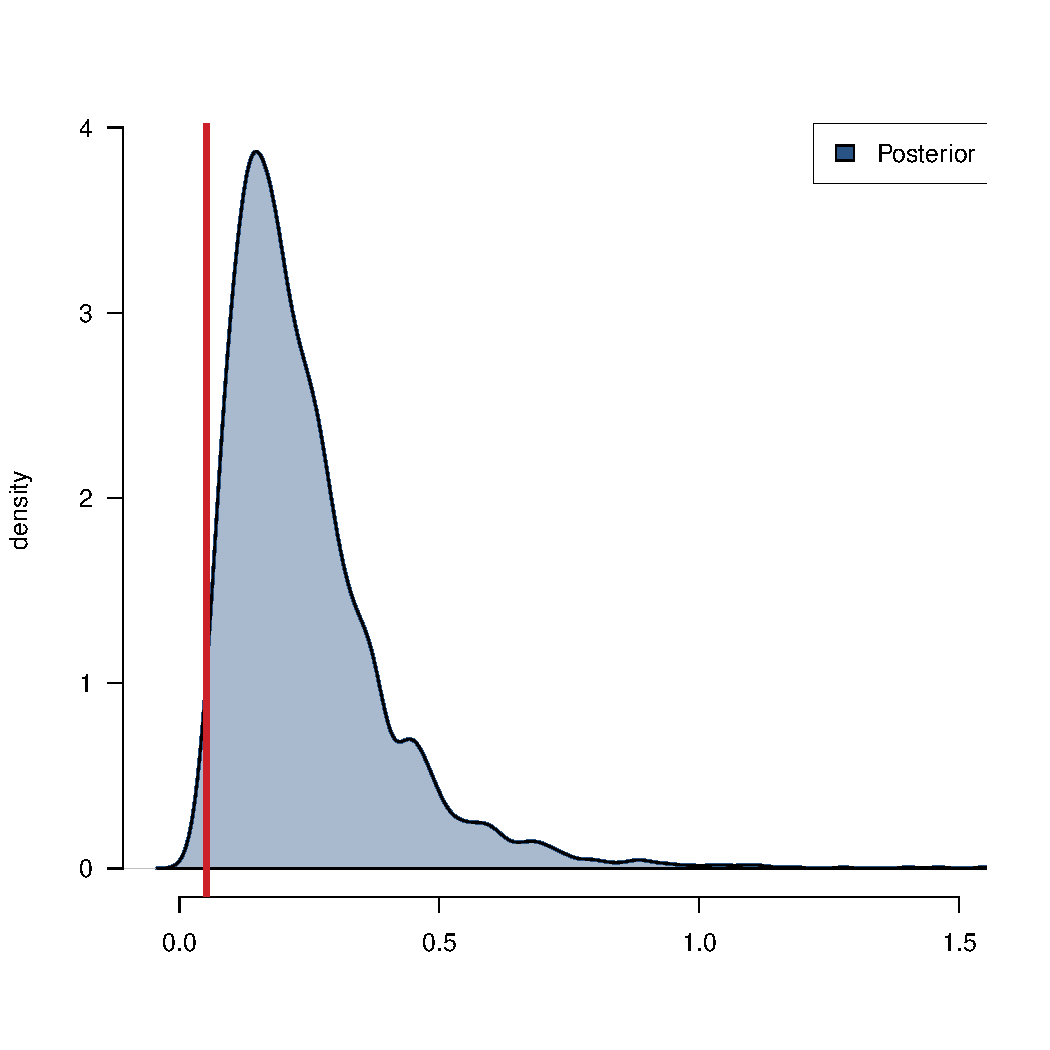
\includegraphics{./Figures/15th-percentile_uncorr.pdf}
		\caption{Uncorrelated model}
	\end{subfigure}
	\caption{Posterior predictions of the product \( Y_1 Y_2 \) for a value sitting around the 15\textup{th} percentile}
	\label{fig::res-15}
\end{figure}

\begin{figure}[htb]
	\centering
	\setkeys{Gin}{width=\linewidth}
	\begin{subfigure}{0.4\textwidth}
		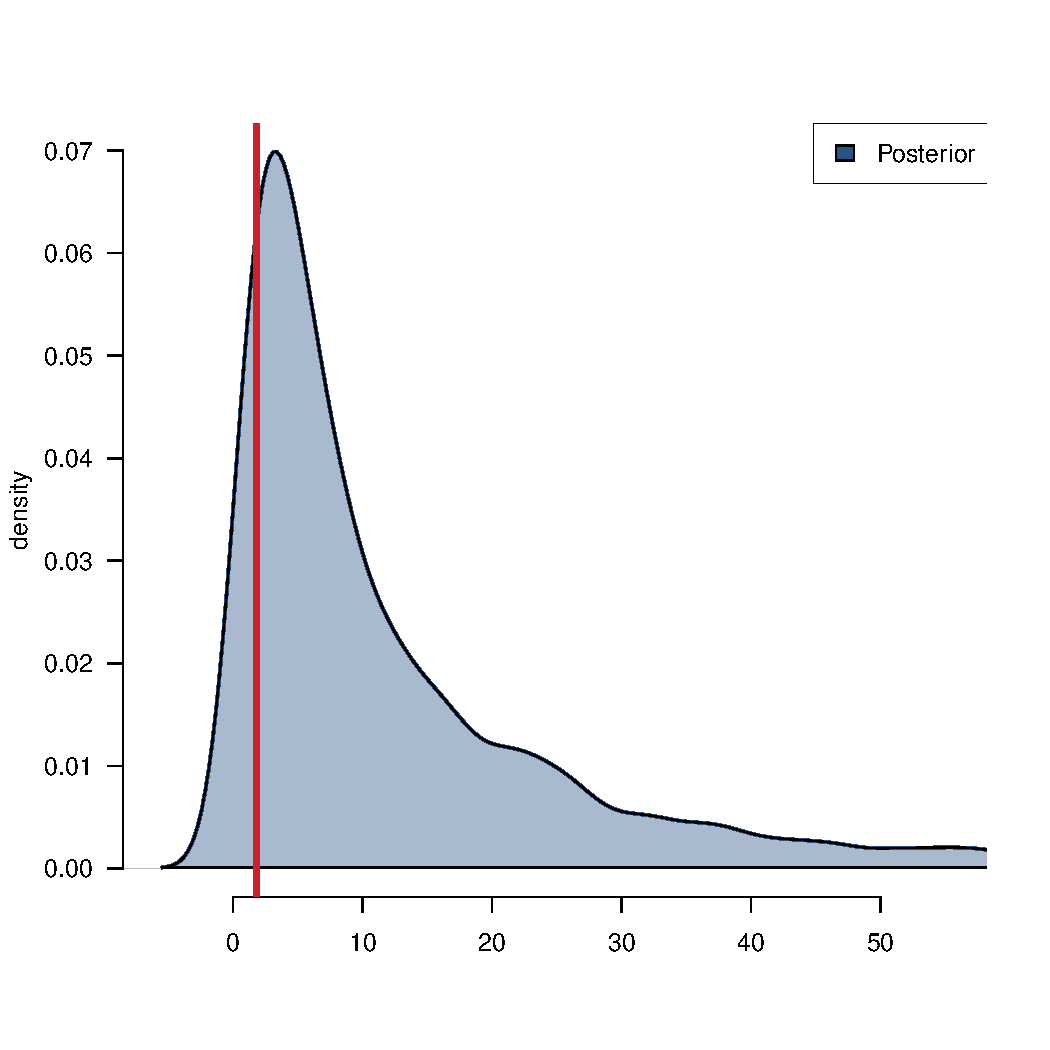
\includegraphics{./Figures/50th-percentile_corr.pdf}
		\caption{Multivariate model}
	\end{subfigure}
	\hfil
	\begin{subfigure}{0.4\textwidth}
		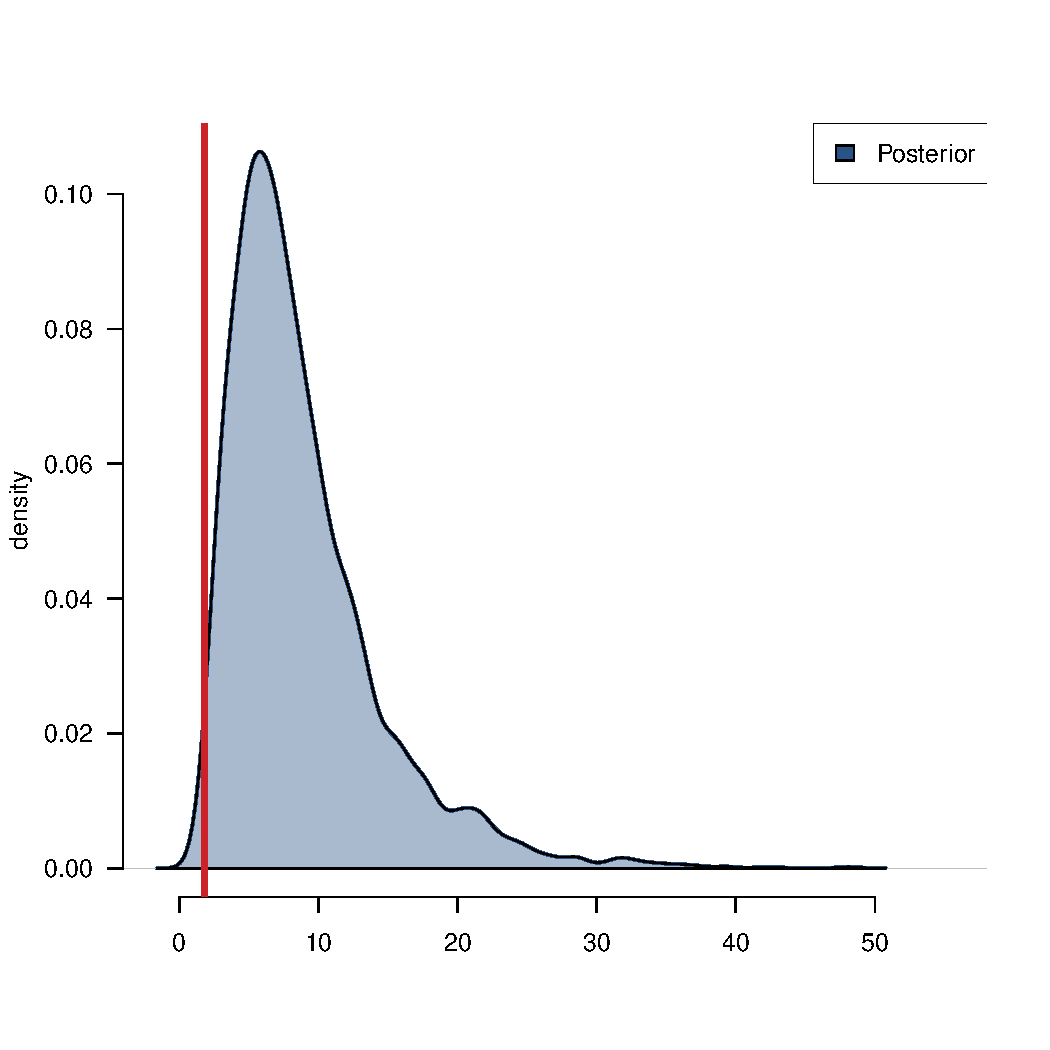
\includegraphics{./Figures/50th-percentile_uncorr.pdf}
		\caption{Uncorrelated model}
	\end{subfigure}
	\caption{Posterior predictions of the product \( Y_1 Y_2 \) for a value sitting around the 50\textup{th} percentile (\ie median)}
	\label{fig::res-50}
\end{figure}

\begin{figure}[htb]
	\centering
	\setkeys{Gin}{width=\linewidth}
	\begin{subfigure}{0.4\textwidth}
		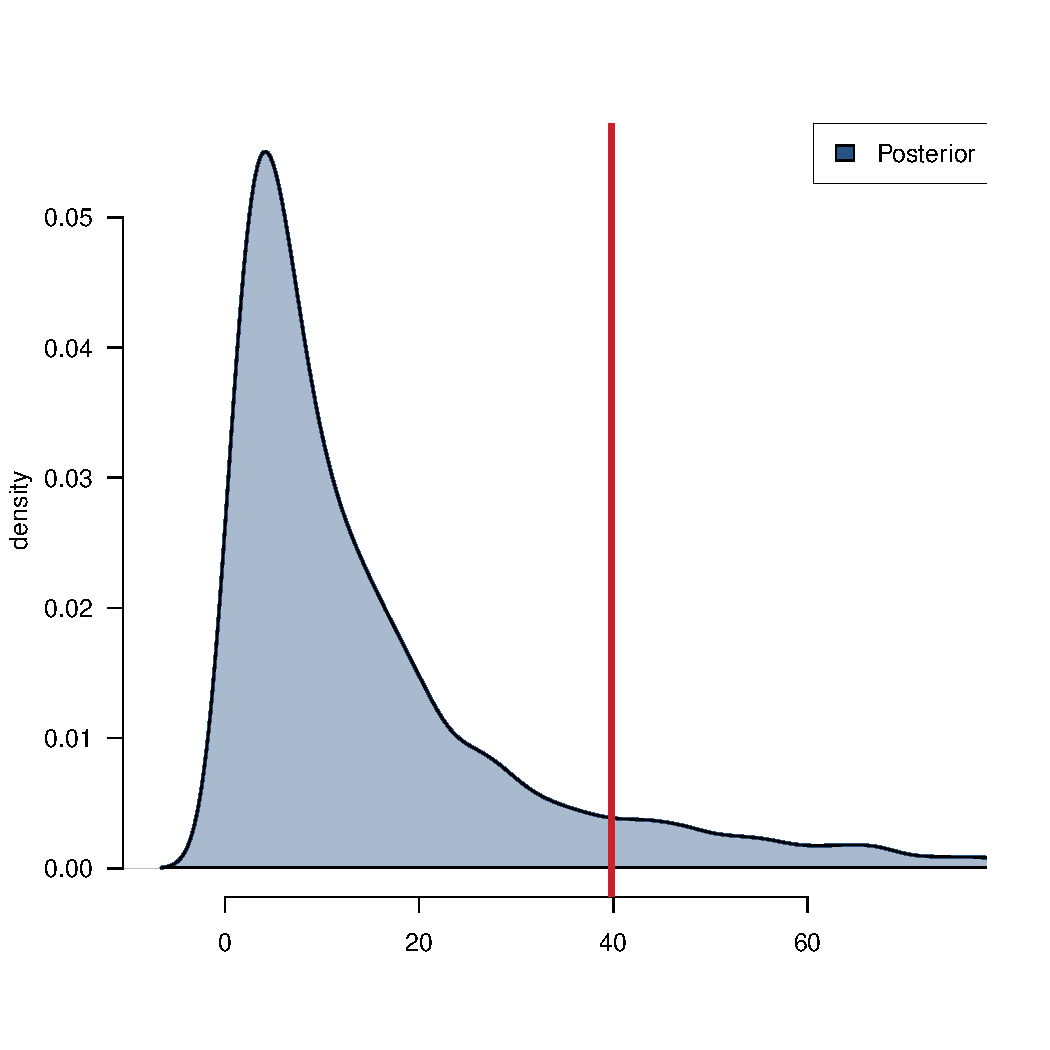
\includegraphics{./Figures/85th-percentile_corr.pdf}
		\caption{Multivariate model}
	\end{subfigure}
	\hfil
	\begin{subfigure}{0.4\textwidth}
		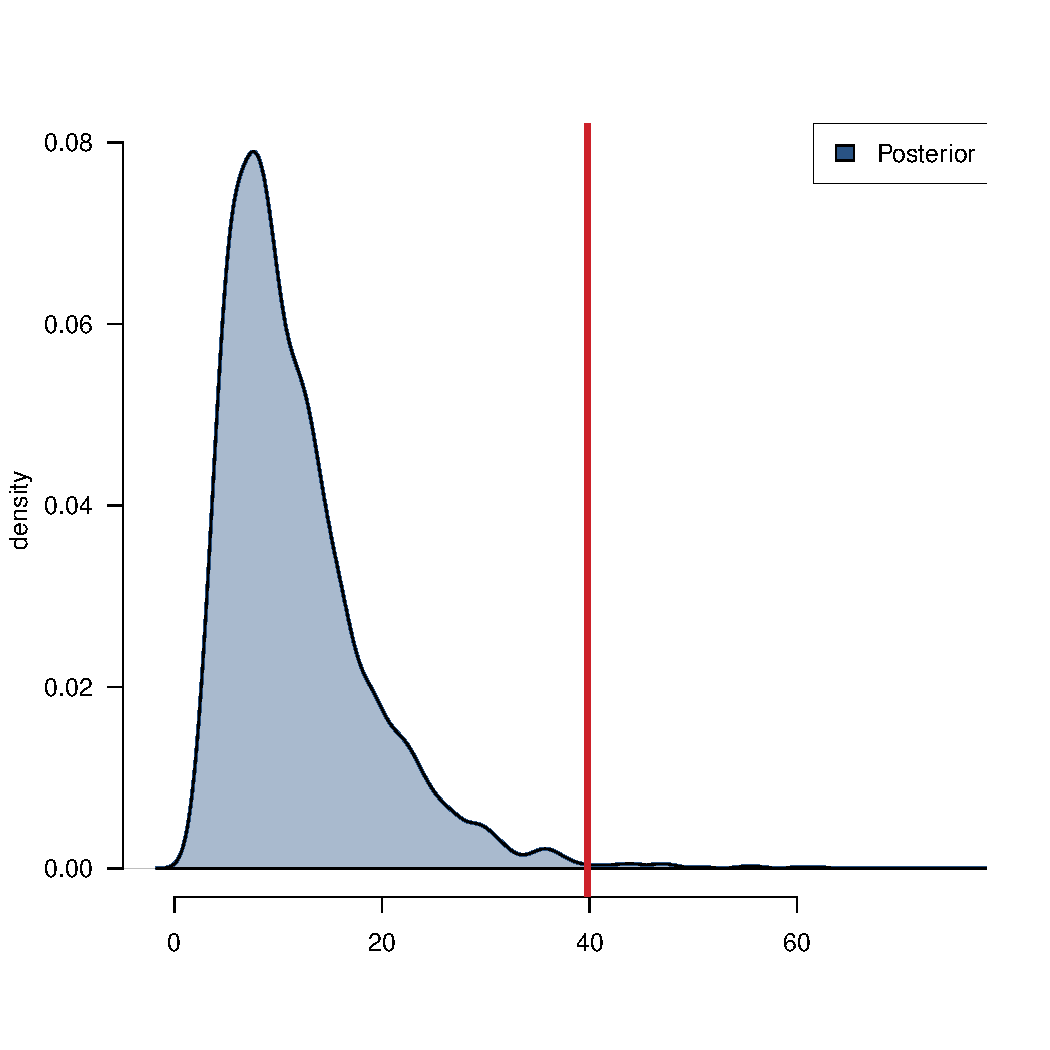
\includegraphics{./Figures/85th-percentile_uncorr.pdf}
		\caption{Uncorrelated model}
	\end{subfigure}
	\caption{Posterior predictions of the product \( Y_1 Y_2 \) for a value sitting around the 85\textup{th} percentile}
	\label{fig::res-85}
\end{figure}

\subsection{Real case study}

I tested a simple multivariate model on \( \logit(r) \) and \( \log(\Vtot) \) with only two intercepts and \( \Sigmabf \) to estimate. I found a positive correlation of 0.28 (0.24 -- 0.31) for \textit{Fagus sylvatica} between the two, suggesting that larger total volumes are predominantly concentrated in the bole.
